\documentclass{standalone}
\usepackage{tikz}
\usetikzlibrary{patterns, positioning}
\usepackage[sfdefault]{ClearSans} %% option 'sfdefault' activates Clear Sans as the default text font
\usepackage[T1]{fontenc}

\begin{document}
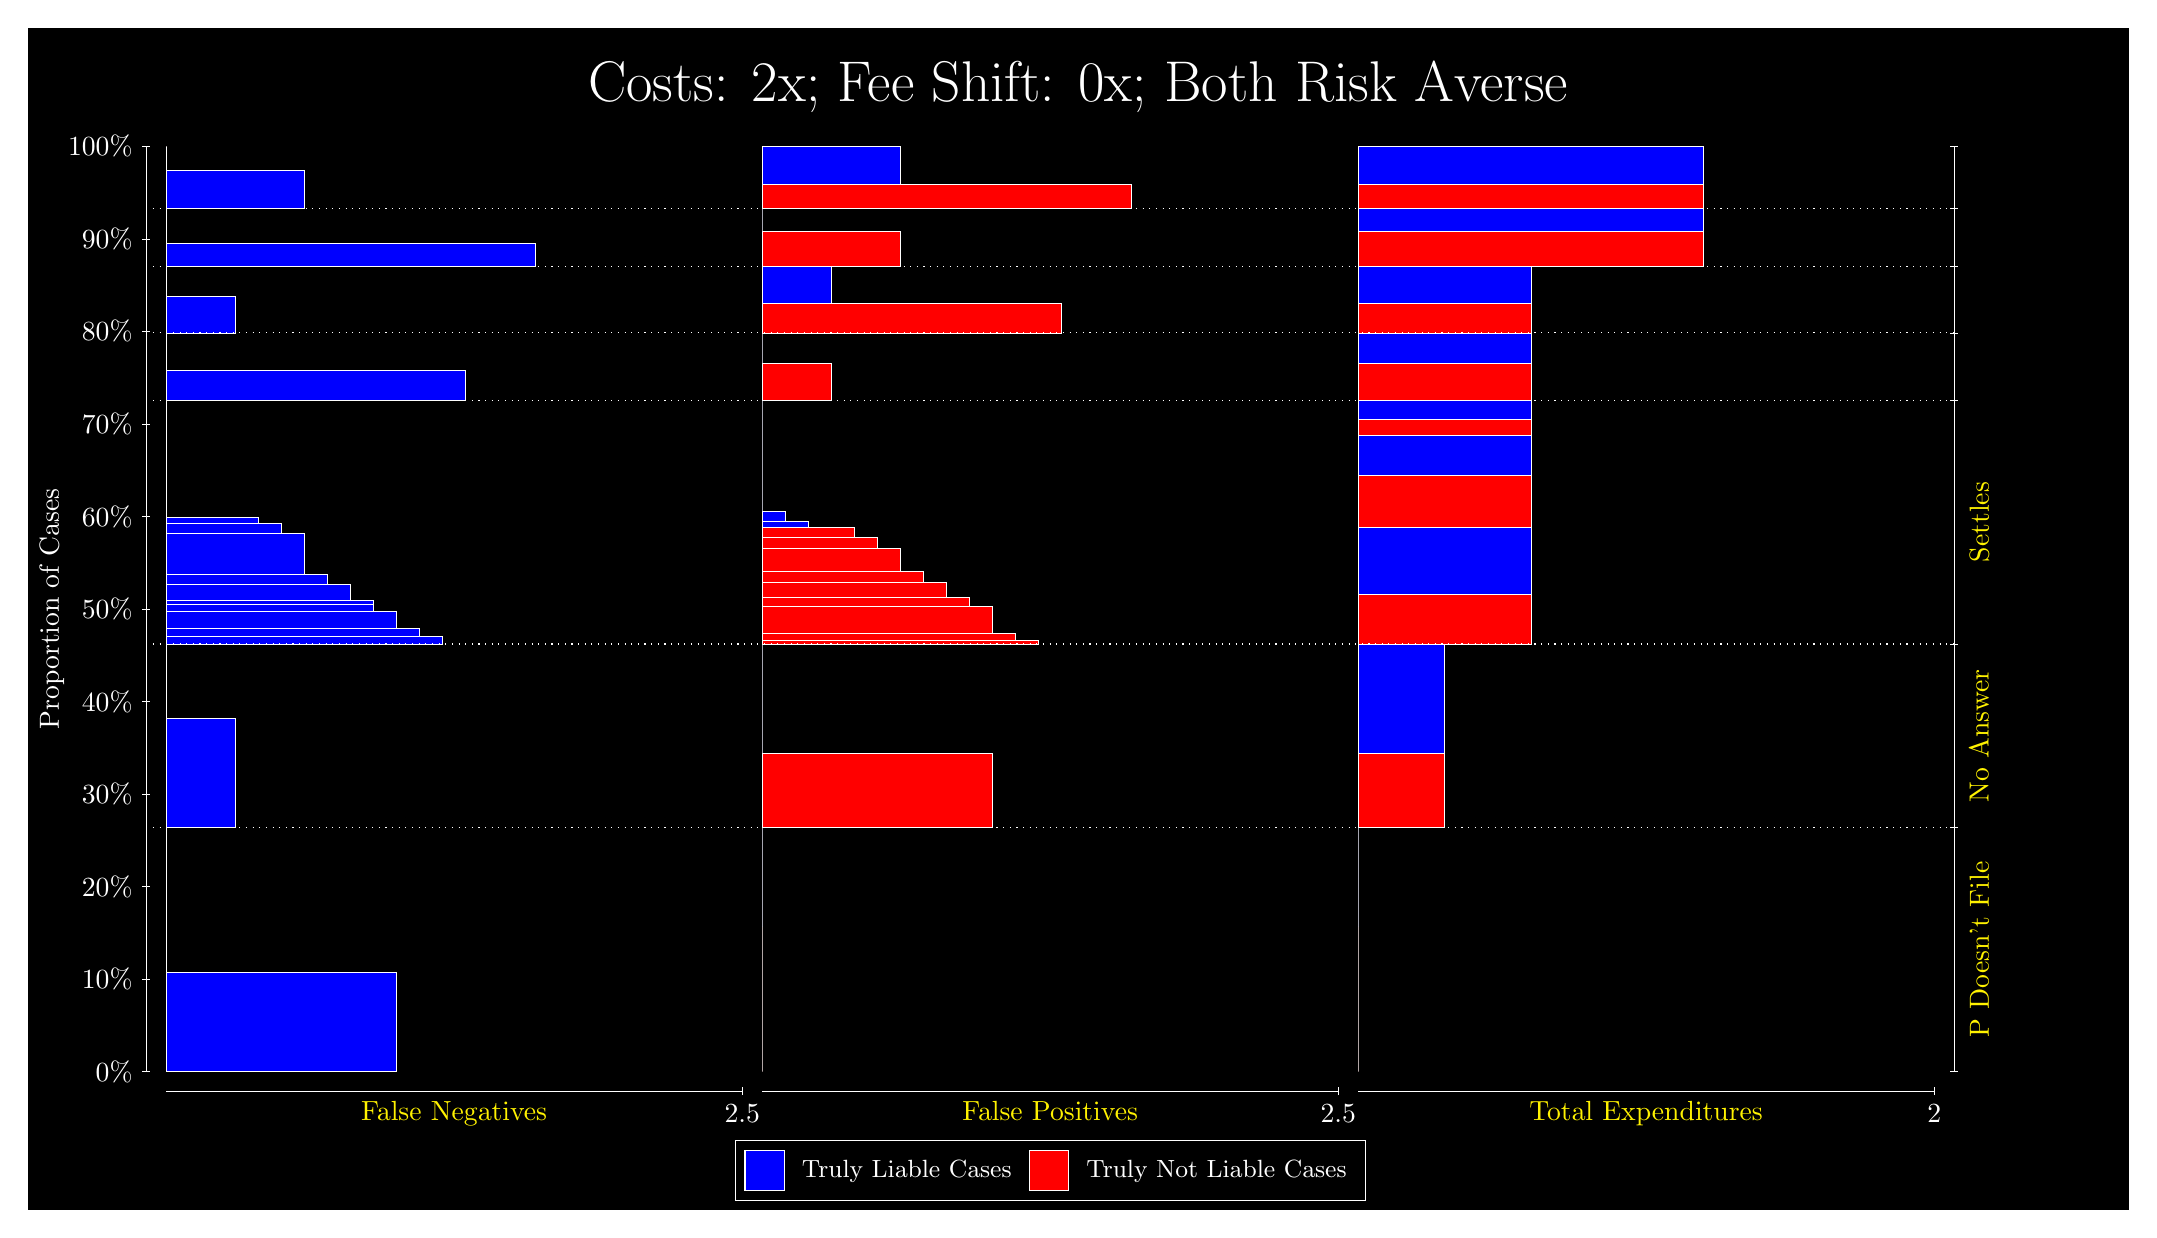
\begin{tikzpicture}
\draw[fill=black] (0,0) rectangle (26.667,15);
\draw[text=white] (0,13.5) rectangle (26.667,15) node[midway] {\huge Costs: 2x; Fee Shift: 0x; Both Risk Averse};
\draw[white, very thin] (1.5,1.75) -- (1.5,13.5);
\node[rotate=90, text=white, anchor=center] at (0.3, 7.625) {Proportion of Cases};
\draw[white, very thin] (1.45,1.75) -- (1.55,1.75);
\node[text=white, anchor=east] at (1.45, 1.75) {0\%};
\draw[white, very thin] (1.45,2.925) -- (1.55,2.925);
\node[text=white, anchor=east] at (1.45, 2.925) {10\%};
\draw[white, very thin] (1.45,4.1) -- (1.55,4.1);
\node[text=white, anchor=east] at (1.45, 4.1) {20\%};
\draw[white, very thin] (1.45,5.275) -- (1.55,5.275);
\node[text=white, anchor=east] at (1.45, 5.275) {30\%};
\draw[white, very thin] (1.45,6.45) -- (1.55,6.45);
\node[text=white, anchor=east] at (1.45, 6.45) {40\%};
\draw[white, very thin] (1.45,7.625) -- (1.55,7.625);
\node[text=white, anchor=east] at (1.45, 7.625) {50\%};
\draw[white, very thin] (1.45,8.8) -- (1.55,8.8);
\node[text=white, anchor=east] at (1.45, 8.8) {60\%};
\draw[white, very thin] (1.45,9.975) -- (1.55,9.975);
\node[text=white, anchor=east] at (1.45, 9.975) {70\%};
\draw[white, very thin] (1.45,11.15) -- (1.55,11.15);
\node[text=white, anchor=east] at (1.45, 11.15) {80\%};
\draw[white, very thin] (1.45,12.325) -- (1.55,12.325);
\node[text=white, anchor=east] at (1.45, 12.325) {90\%};
\draw[white, very thin] (1.45,13.5) -- (1.55,13.5);
\node[text=white, anchor=east] at (1.45, 13.5) {100\%};

\draw[white, very thin] (24.457,1.75) -- (24.457,13.5);
\draw[white, very thin] (24.407,1.75) -- (24.507,1.75);
\node[anchor=west] at (24.407, 1.75) {};
\draw[white, very thin] (24.407,4.8475) -- (24.507,4.8475);
\node[anchor=west] at (24.407, 4.8475) {};
\draw[white, very thin] (24.407,7.1798) -- (24.507,7.1798);
\node[anchor=west] at (24.407, 7.1798) {};
\draw[white, very thin] (24.407,10.275) -- (24.507,10.275);
\node[anchor=west] at (24.407, 10.275) {};
\draw[white, very thin] (24.407,11.131) -- (24.507,11.131);
\node[anchor=west] at (24.407, 11.131) {};
\draw[white, very thin] (24.407,11.977) -- (24.507,11.977);
\node[anchor=west] at (24.407, 11.977) {};
\draw[white, very thin] (24.407,12.712) -- (24.507,12.712);
\node[anchor=west] at (24.407, 12.712) {};
\draw[white, very thin] (24.407,13.5) -- (24.507,13.5);
\node[anchor=west] at (24.407, 13.5) {};

\draw[white, very thin, fill=blue] (1.75,1.75) rectangle (4.6775,3.0108);
\draw[white, very thin, fill=red] (1.75,3.0108) rectangle (1.75,4.8475);
\draw[white, very thin, fill=blue] (1.75,4.8475) rectangle (2.6283,6.2346);
\draw[white, very thin, fill=red] (1.75,6.2346) rectangle (1.75,7.1798);
\draw[white, very thin, fill=blue] (1.75,7.1798) rectangle (5.2631,7.2774);
\draw[white, very thin, fill=blue] (1.75,7.2774) rectangle (4.9703,7.3758);
\draw[white, very thin, fill=blue] (1.75,7.3758) rectangle (4.6775,7.59);
\draw[white, very thin, fill=blue] (1.75,7.59) rectangle (4.3848,7.6894);
\draw[white, very thin, fill=blue] (1.75,7.6894) rectangle (4.3848,7.7373);
\draw[white, very thin, fill=blue] (1.75,7.7373) rectangle (4.092,7.9437);
\draw[white, very thin, fill=blue] (1.75,7.9437) rectangle (3.7993,8.0663);
\draw[white, very thin, fill=blue] (1.75,8.0663) rectangle (3.5065,8.5897);
\draw[white, very thin, fill=blue] (1.75,8.5897) rectangle (3.2138,8.7185);
\draw[white, very thin, fill=blue] (1.75,8.7185) rectangle (2.921,8.7867);
\draw[white, very thin, fill=red] (1.75,8.7867) rectangle (1.75,10.275);
\draw[white, very thin, fill=blue] (1.75,10.275) rectangle (5.5558,10.659);
\draw[white, very thin, fill=red] (1.75,10.659) rectangle (1.75,11.131);
\draw[white, very thin, fill=blue] (1.75,11.131) rectangle (2.6283,11.596);
\draw[white, very thin, fill=red] (1.75,11.596) rectangle (1.75,11.977);
\draw[white, very thin, fill=blue] (1.75,11.977) rectangle (6.4341,12.269);
\draw[white, very thin, fill=red] (1.75,12.269) rectangle (1.75,12.712);
\draw[white, very thin, fill=blue] (1.75,12.712) rectangle (3.5065,13.191);
\draw[white, very thin, fill=red] (1.75,13.191) rectangle (1.75,13.5);
\draw[white, very thin, fill=red] (9.3189,1.75) rectangle (9.3189,3.5867);
\draw[white, very thin, fill=blue] (9.3189,3.5867) rectangle (9.3189,4.8475);
\draw[white, very thin, fill=red] (9.3189,4.8475) rectangle (12.246,5.7927);
\draw[white, very thin, fill=blue] (9.3189,5.7927) rectangle (9.3189,7.1798);
\draw[white, very thin, fill=red] (9.3189,7.1798) rectangle (12.832,7.2249);
\draw[white, very thin, fill=red] (9.3189,7.2249) rectangle (12.539,7.3111);
\draw[white, very thin, fill=red] (9.3189,7.3111) rectangle (12.246,7.6571);
\draw[white, very thin, fill=red] (9.3189,7.6571) rectangle (11.954,7.7693);
\draw[white, very thin, fill=red] (9.3189,7.7693) rectangle (11.661,7.9634);
\draw[white, very thin, fill=red] (9.3189,7.9634) rectangle (11.368,8.0995);
\draw[white, very thin, fill=red] (9.3189,8.0995) rectangle (11.075,8.3964);
\draw[white, very thin, fill=red] (9.3189,8.3964) rectangle (10.783,8.5293);
\draw[white, very thin, fill=red] (9.3189,8.5293) rectangle (10.49,8.6681);
\draw[white, very thin, fill=blue] (9.3189,8.6681) rectangle (9.9044,8.7364);
\draw[white, very thin, fill=blue] (9.3189,8.7364) rectangle (9.6116,8.8652);
\draw[white, very thin, fill=blue] (9.3189,8.8652) rectangle (9.3189,10.275);
\draw[white, very thin, fill=red] (9.3189,10.275) rectangle (10.197,10.748);
\draw[white, very thin, fill=blue] (9.3189,10.748) rectangle (9.3189,11.131);
\draw[white, very thin, fill=red] (9.3189,11.131) rectangle (13.125,11.512);
\draw[white, very thin, fill=blue] (9.3189,11.512) rectangle (10.197,11.977);
\draw[white, very thin, fill=red] (9.3189,11.977) rectangle (11.075,12.42);
\draw[white, very thin, fill=blue] (9.3189,12.42) rectangle (9.3189,12.712);
\draw[white, very thin, fill=red] (9.3189,12.712) rectangle (14.003,13.021);
\draw[white, very thin, fill=blue] (9.3189,13.021) rectangle (11.075,13.5);
\draw[white, very thin, fill=red] (16.888,1.75) rectangle (16.888,3.5867);
\draw[white, very thin, fill=blue] (16.888,3.5867) rectangle (16.888,4.8475);
\draw[white, very thin, fill=red] (16.888,4.8475) rectangle (17.986,5.7927);
\draw[white, very thin, fill=blue] (16.888,5.7927) rectangle (17.986,7.1798);
\draw[white, very thin, fill=red] (16.888,7.1798) rectangle (19.083,7.8061);
\draw[white, very thin, fill=blue] (16.888,7.8061) rectangle (19.083,8.6646);
\draw[white, very thin, fill=red] (16.888,8.6646) rectangle (19.083,9.32);
\draw[white, very thin, fill=blue] (16.888,9.32) rectangle (19.083,9.8297);
\draw[white, very thin, fill=red] (16.888,9.8297) rectangle (19.083,10.036);
\draw[white, very thin, fill=blue] (16.888,10.036) rectangle (19.083,10.275);
\draw[white, very thin, fill=red] (16.888,10.275) rectangle (19.083,10.748);
\draw[white, very thin, fill=blue] (16.888,10.748) rectangle (19.083,11.131);
\draw[white, very thin, fill=red] (16.888,11.131) rectangle (19.083,11.512);
\draw[white, very thin, fill=blue] (16.888,11.512) rectangle (19.083,11.977);
\draw[white, very thin, fill=red] (16.888,11.977) rectangle (21.279,12.42);
\draw[white, very thin, fill=blue] (16.888,12.42) rectangle (21.279,12.712);
\draw[white, very thin, fill=red] (16.888,12.712) rectangle (21.279,13.021);
\draw[white, very thin, fill=blue] (16.888,13.021) rectangle (21.279,13.5);
\draw[white, dotted] (1.5,4.8475) -- (24.457,4.8475);
\draw[white, dotted] (1.5,7.1798) -- (24.457,7.1798);
\draw[white, dotted] (1.5,10.275) -- (24.457,10.275);
\draw[white, dotted] (1.5,11.131) -- (24.457,11.131);
\draw[white, dotted] (1.5,11.977) -- (24.457,11.977);
\draw[white, dotted] (1.5,12.712) -- (24.457,12.712);
\draw[white, very thin] (1.75,1.5) -- (9.0689,1.5);
\node[text=yellow, anchor=north] at (5.4094, 1.5) {False Negatives};
\draw[white, very thin] (9.0689,1.45) -- (9.0689,1.55);
\node[text=white, anchor=north] at (9.0689, 1.45) {2.5};

\draw[white, very thin] (9.3189,1.5) -- (16.638,1.5);
\node[text=yellow, anchor=north] at (12.978, 1.5) {False Positives};
\draw[white, very thin] (16.638,1.45) -- (16.638,1.55);
\node[text=white, anchor=north] at (16.638, 1.45) {2.5};

\draw[white, very thin] (16.888,1.5) -- (24.207,1.5);
\node[text=yellow, anchor=north] at (20.547, 1.5) {Total Expenditures};
\draw[white, very thin] (24.207,1.45) -- (24.207,1.55);
\node[text=white, anchor=north] at (24.207, 1.45) {2};

\node[text=yellow, centered, rotate=90] at (24.777, 3.2988) {P Doesn't File};
\node[text=yellow, centered, rotate=90] at (24.777, 6.0137) {No Answer};
\node[text=yellow, centered, rotate=90] at (24.777, 8.7274) {Settles};





\draw (12.978300999999998,1.5) node[draw=none] (baseCoordinate) {};
\begin{scope}[align=center]
        \matrix[scale=0.5, draw=white, below=0.5cm of baseCoordinate, nodes={draw}, column sep=0.1cm]{
            \node[rectangle, draw, minimum width=0.5cm, minimum height=0.5cm, fill=blue] {}; &
            \node[draw=none, font=\small, text=white] (B) {Truly Liable Cases}; &
            \node[rectangle, draw, minimum width=0.5cm, minimum height=0.5cm, fill=red] {}; &
            \node[draw=none, font=\small, text=white] (B) {Truly Not Liable Cases}; \\
            };
\end{scope}

\end{tikzpicture}
\end{document}